\documentclass{article}

\usepackage{amsmath}
\usepackage{graphicx}
\usepackage{float}
\usepackage{hyperref}
\usepackage{fancyhdr}
\usepackage[a4paper, margin=1in]{geometry}

\title{Experiment Report: Image Processing with OpenMV H7}
\author{Ziqi Wang}
\date{\today}

\pagestyle{fancy}
\fancyhead{}
\fancyfoot{}
\fancyfoot[R]{\thepage}

\begin{document}

\maketitle

\section{Introduction}
This experiment demonstrates three tasks using the OpenMV H7 board with the STM32H7 processor. The tasks are:
\begin{enumerate}
    \item Lighting up LEDs.
    \item Drawing circles on detected blue color blocks.
    \item Using two servos to track a blue color block and keep it centered on the screen.
\end{enumerate}

The OpenMV H7 is a powerful microcontroller board designed for image processing applications. It uses an ARM Cortex-M7 processor, which allows for real-time computer vision tasks. This experiment explores the capabilities of the OpenMV H7 board and showcases practical applications of image processing and servo control.

\section{Equipment}
\begin{itemize}
    \item OpenMV H7 board
    \item LEDs
    \item Two servos
    \item Blue object for color tracking
\end{itemize}

\section{Task 1: Lighting up LEDs}
\subsection{Implementation}
To light up LEDs connected to the OpenMV H7, we use the \texttt{pyb} module which provides control over the board's peripherals. The following code snippet initializes and blinks three LEDs in sequence:
\begin{verbatim}
import time
from pyb import LED

# Initialize LEDs
red_led = LED(1)    # Red LED
green_led = LED(2)  # Green LED
blue_led = LED(3)   # Blue LED

# Function to blink LED
def blink_led(led, duration):
    led.on()
    time.sleep(duration)
    led.off()
    time.sleep(duration)

while True:
    blink_led(red_led, 1)
    blink_led(blue_led, 1)
    blink_led(green_led, 1)
\end{verbatim}

\subsection{Theory}
LEDs are controlled by toggling the GPIO pins on the microcontroller. By setting the pin high, current flows through the LED, causing it to emit light. The \texttt{time.sleep} function introduces a delay to create a blinking effect.

\begin{figure}[H]
    \centering
    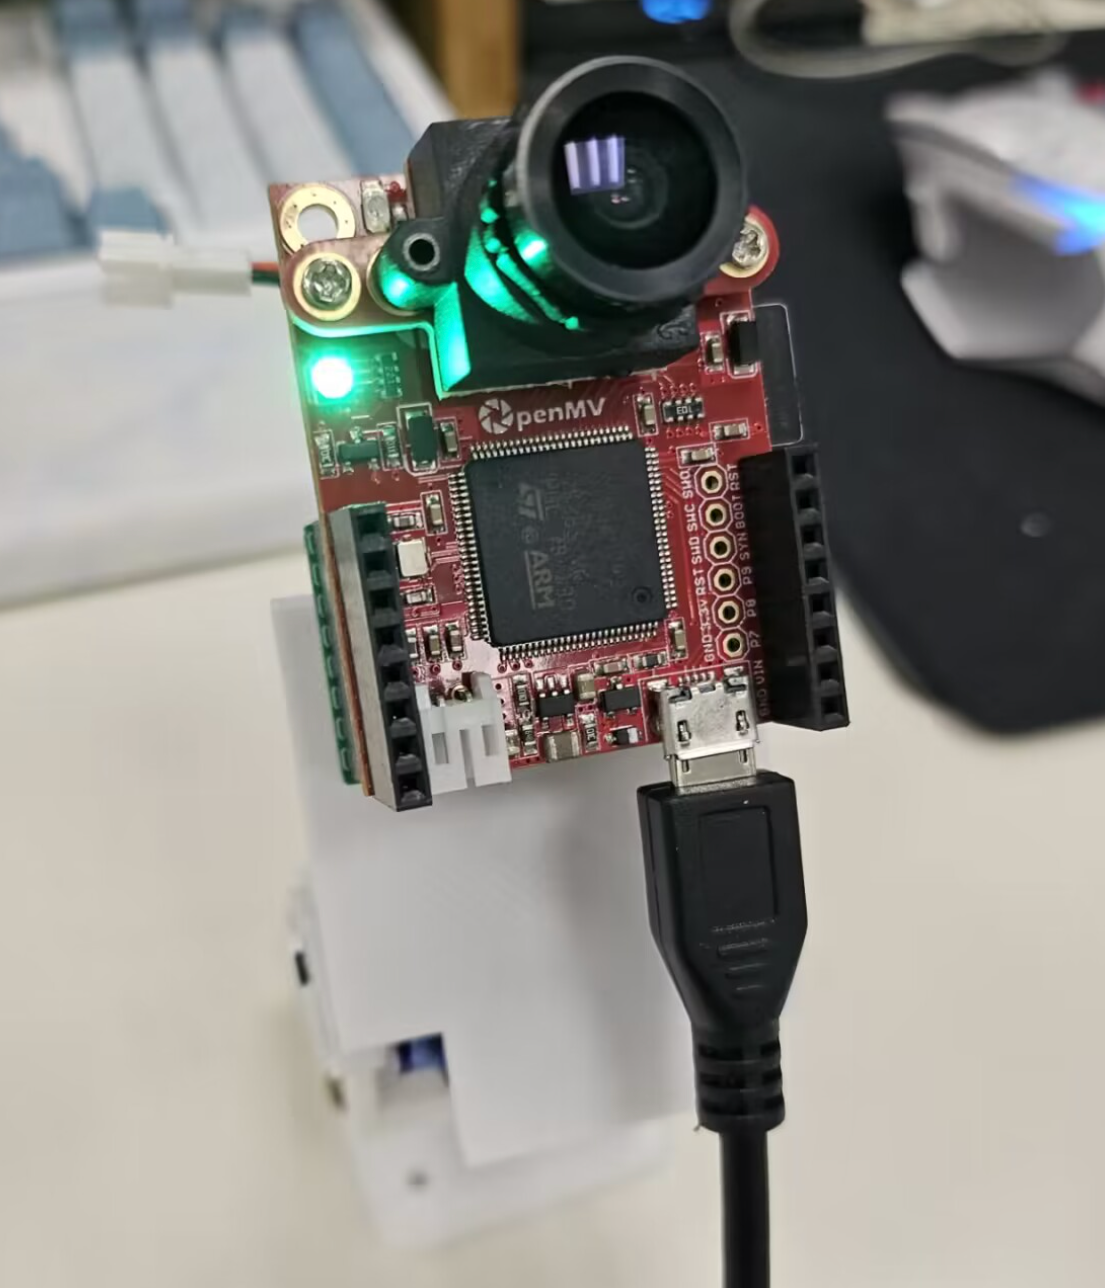
\includegraphics[width=0.5\textwidth]{LED.png}
    \caption{LED setup on the OpenMV H7 board}
\end{figure}

\section{Task 2: Drawing Circles on Detected Blue Color Blocks}
\subsection{Implementation}
Using the OpenMV H7's image processing capabilities, we detect blue color blocks and draw circles around them. The following code snippet demonstrates this:
\begin{verbatim}
import sensor, image, time, math

threshold_index = 2  # 0 for red, 1 for green, 2 for blue

# Color Tracking Thresholds (L Min, L Max, A Min, A Max, B Min, B Max)
thresholds = [
    (30, 100, 15, 127, 15, 127),  # generic_red_thresholds
    (30, 100, -64, -8, -32, 32),  # generic_green_thresholds
    (0, 30, 0, 64, -128, 0),      # generic_blue_thresholds
]

sensor.reset()
sensor.set_pixformat(sensor.RGB565)
sensor.set_framesize(sensor.QVGA)
sensor.skip_frames(time=2000)
sensor.set_auto_gain(False)  # must be turned off for color tracking
sensor.set_auto_whitebal(False)  # must be turned off for color tracking
clock = time.clock()

while True:
    clock.tick()
    img = sensor.snapshot()
    for blob in img.find_blobs(
        [thresholds[threshold_index]],
        pixels_threshold=200,
        area_threshold=200,
        merge=True,
    ):
        img.draw_circle(blob.cx(), blob.cy(),  \
            int(math.sqrt(blob.area()/math.pi)), color=(0, 0, 255))
        img.draw_cross(blob.cx(), blob.cy())
    print(clock.fps())
\end{verbatim}

\subsection{Theory}
Color detection is based on the LAB color space, which separates the lightness component from the color components, making it easier to segment specific colors under varying lighting conditions. The \texttt{find\_blobs} method identifies regions in the image that match the specified color threshold, and we use \texttt{draw\_circle} to highlight these regions.

\begin{figure}[H]
    \centering
    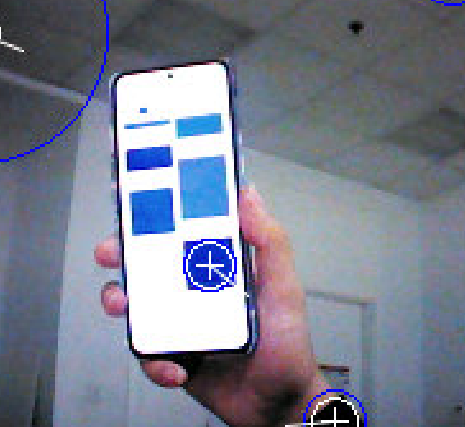
\includegraphics[width=0.5\textwidth]{blue_track.png}
    \caption{Blue color block detection and circle drawing}
\end{figure}

\section{Task 3: Tracking Blue Color Block with Servos}
\subsection{Implementation}
To keep a blue color block centered on the screen, we use two servos to adjust the camera's orientation. The following code combines color tracking with servo control:
\begin{verbatim}
import sensor, image, time, math
from pyb import Servo

# Initialize servos
sy = Servo(1)  # Y direction servo
sx = Servo(2)  # X direction servo

threshold_index = 2  # 0 for red, 1 for green, 2 for blue

# Color Tracking Thresholds (L Min, L Max, A Min, A Max, B Min, B Max)
thresholds = [
    (30, 100, 15, 127, 15, 127),  # generic_red_thresholds
    (30, 100, -64, -8, -32, 32),  # generic_green_thresholds
    (0, 30, 0, 64, -128, 0)       # generic_blue_thresholds
]

sensor.reset()
sensor.set_pixformat(sensor.RGB565)
sensor.set_framesize(sensor.QVGA)
sensor.skip_frames(time=2000)
sensor.set_auto_gain(False)  # must be turned off for color tracking
sensor.set_auto_whitebal(False)  # must be turned off for color tracking
clock = time.clock()

center_x = 160
center_y = 120

sx.angle(0)
sy.angle(0)

while True:
    clock.tick()
    img = sensor.snapshot()
    blobs = img.find_blobs(
        [thresholds[threshold_index]],
        pixels_threshold=200,
        area_threshold=200,
        merge=True,
    )
    if blobs:
        largest_blob = max(blobs, key=lambda b: b.pixels())
        blob_x = largest_blob.cx()
        blob_y = largest_blob.cy()
        offset_x = blob_x - center_x
        offset_y = blob_y - center_y

        img.draw_circle(largest_blob.cx(), largest_blob.cy(), \
            int(math.sqrt(largest_blob.area()/math.pi)), color=(0, 0, 255))
        img.draw_cross(largest_blob.cx(), largest_blob.cy())

        if abs(offset_x) > 10:
            new_sx_angle = sx.angle() - offset_x * 0.1
            new_sx_angle = max(min(new_sx_angle, 90), -90)
            sx.angle(new_sx_angle)

        if abs(offset_y) > 10:
            new_sy_angle = sy.angle() + offset_y * 0.1
            new_sy_angle = max(min(new_sy_angle, 90), -90)
            sy.angle(new_sy_angle)

    print(clock.fps())
\end{verbatim}

\subsection{Theory}
Servo motors are used to adjust the camera's orientation. By calculating the offset between the detected color block's center and the screen center, we can adjust the servos to minimize this offset, thereby keeping the color block centered. This involves a basic form of feedback control, where the servos' angles are updated based on the position error.

\section{Conclusion}
This experiment successfully demonstrated the use of the OpenMV H7 board for lighting up LEDs, detecting and drawing on color blocks, and implementing a basic tracking system using servos. The combination of image processing and servo control illustrates the powerful capabilities of the OpenMV H7 for real-time embedded vision applications.

By leveraging the STM32H7 processor's performance, the OpenMV H7 can handle complex tasks that involve both high-speed image processing and precise motor control, making it an ideal platform for robotics and automation projects.

\end{document}
